%%%%%%%%%%%%%%%%%%%%%%%%%%%%%%%%%%%%%%%%%%%%%%%%%%%%%%%%%%%%%%%%%%%%%%%%%%%%%%%%
%2345678901234567890123456789012345678901234567890123456789012345678901234567890
%        1         2         3         4         5         6         7         8


%\documentclass[twocolumn,journal]{IEEEtran}
\documentclass[conference]{IEEEtran}
%\documentclass[letterpaper, 10 pt, conference]{ieeeconf}  % Comment t                                                      his line out
                                                          % if you need a4paper
%\documentclass[a4paper, 10pt, conference]{ieeeconf}      % Use this line for a4
                                                          % paper

\IEEEoverridecommandlockouts                           % This command is only
                                                          % needed if you want to
                                                          % use the \thanks command
\overrideIEEEmargins
% See the \addtolength command later in the file to balance the column lengths
% on the last page of the document

\newtheorem{theorem}{Theorem}
\newtheorem{definition}{Definition}
\newtheorem{corollary}{Corollary}
\newtheorem{example}{Example}
\newtheorem{assumption}{Assumption}
\newtheorem{hypothesis}{Hypothesis}
\newtheorem{lemma}{Lemma}
\newtheorem{remark}{Remark}
\newtheorem{notation}{Notation}
\newtheorem{algorithm}{Algorithm}
\newtheorem{property}{Property}
%\newcommand{\for}{\textbf{for}}
%\newcommand{\STATE}{\quad}
% The following packages can be found on http:\\www.ctan.org
\usepackage{graphicx}
\usepackage{subfig}% for pdf, bitmapped graphics files
%\usepackage{epsfig} % for postscript graphics files
\usepackage{mathptmx} % assumes new font selection scheme installed
\usepackage{times} % assumes new font selection scheme installed
\usepackage{amsmath} % assumes amsmath package installed
\usepackage{amssymb}  % assumes amsmath package installed
\usepackage{algorithm}
\usepackage{algorithmic}
\usepackage{multirow}
\usepackage{amsmath}
\usepackage{xcolor}

\title{\LARGE \bf
Stability of $(n,k)$ nonlinear feedback shift registers}

\author{Meilin Li, Jianquan Lu
%\thanks{This work was supported by the National Natural Science Foundation of China under Grant No. 61573102, and China Postdoctoral Science Foundation under Grant No. 2014M560377 and 2015T80483, and Jiangsu Province Six Talent Peaks Project under Grant 2015-ZNDW-002. }%
\thanks{Meilin Li is with the School of Mathematics, Southeast
University, Nanjing 210096, China {\tt\small 220151318@seu.edu.cn}}
\thanks{Jianquan Lu is with the School of Mathematics, Southeast
University, Nanjing 210096, China
{\tt\small jqluma@seu.edu.cn}}}
%\thanks{Tingwen Huang is with Texas AM University at Qatar, Dc/o Qatar Foundation, PO Box 5825, Doha, Qatar}
%\thanks{ Jinde Cao is
%with the Department of Mathematics, Southeast University, Nanjing
%210096, China {\tt\small jdcao@seu.edu.cn}}
%\thanks{}
%\thanks{}
%\thanks{} }
\begin{document}

\maketitle
\thispagestyle{empty}
\pagestyle{empty}

%\usepackage[a4paper,left=2.1cm,right=2.1cm,top=2.2cm,bottom=2.2cm]{geometry}
%%%%%%%%%%%%%%%%%%%%%%%%%%%%%%%%%%%%%%%%%%%%%%%%%%%%%%%%%%%%%%%%%%%%%%%%%%%%%%%%
\begin{abstract}
In this paper, the $(n,k)$ nonlinear feedback shift register (NFSR) is regarded as a Boolean network (BN). Semi-tensor product (STP) of matrices is used to convert $(n,k)$ NFSR into an equivalent algebraic equation. Based on STP of matrices, a novel way is proposed to study stability of $(n,k)$ NFSR and the periodicity of $(n,k)$ NFSR. First, the stability of the $(n,k)$ NFSR is investigated, and we propose an algorithm to judge the stability of an $(n,k)$ NFSR. Second, we reveal relationship between the minimal period of output sequence of a cycle for an $(n,k)$ NFSR and the length of the cycle. Third, we investigate the period of $(n,k)$ NFSR. Some existing methods can only be used to investigate the cycle of the $(n,k)$ NFSR, while in this paper, we can simultaneously investigate stability of an $(n,k)$ NFSR and the period of $(n,k)$ NFSR by using the method of STP.
\end{abstract}

\begin{keywords}
$(n,k)$ NFSR, stability, minimal period, period, semi-tensor product, Boolean networks
\end{keywords}

\section{introduction}
Information security is very important for our society. There are many confidential information about financial status, research, products for different organizations. In order to protect the confidential information from leakage, the stream cipher has been widely used in encryption \cite{Golomb2002Shift}. The main building blocks of stream cipher is nonlinear feedback shift registers (NFSR). NFSR can produce pseudo-random sequences.

There are two types of NFSR: (1) Fibonacci NFSR; (2) Galois NFSR. Fibonacci NFSR is shown in Fig.\ref{fsr}. Fibonacci NFSR consists $n$ binary storage elements from left to right as $n-1,n-2,...,1,0$. The value of the $i$-th $(0\leq i\leq n-2)$ bit is updated by the value of $(i+1)$-th bit, and the value of $(n-1)$-th bit is updated by feedback function $f$ which depends on values of bits of $0,1,...,n-1$.While the Galois NFSR shown in Fig.\ref{gsr} is different from Fibonacci NFSR. In Galois NFSR, the value of every bit is updated by its own feedback function which at most relate to every bit. In order to improve the speed of output sequence generation, E. Dubrova proposed a new type of NFSR named $(n,k)$ NFSR in \cite{Dubrova2008On}. The period of Fibonacci NFSR is equal to the largest length of its state cycle. An $(n,k)$ NFSR can be considered as a generalization of the Galois NFSR. In an $(n,k)$ NFSR, every bit is updated by a feedback function, which is a nonlinear function relating to value of $(i+1)mod~n$-th bit and up to values of $k-1$ other bits. But there is a weakness for the $(n,k)$ NFSR. The period of an $(n,k)$ NFSR is not necessary equal to the length of longest cycle of $(n,k)$ NFSR, and this would cause some problems to observe the period of output sequences of an $(n,k)$ NFSR. 

In order to solve the above mentioned problems, in this paper, we provide a new method to investigate the period of output sequences of a cycle of an $(n,k)$ NFSR by using the method of semi-tensor product (STP) of matrices. The method of STP was proposed by Cheng \textit{et al.} in \cite{Cheng2011Analysis}. After the proposal of method of STP, it has been used in many fields, such as large-scale systems \cite{Zhao2013Aggregation}, graph coloring \cite{Wang2012A}\cite{Zhong2015Finding}, Petri nets \cite{Han2015Calculation}, Boolean networks (BNs) \cite{Guo2015Set}\cite{Fornasini2013On} and NFSR \cite{Zhong2014Stability}\cite{Zhao2014Novel}. By using the method of STP, some fundamental problems of BNs have been solved,
such as synchronization \cite{Zhong2014Synchronization}\cite{Zhang2014Synchronization}, stability \cite{Liu2016Sampled}\cite{Li2014Stability}\cite{Fornasini2013On}, stabilization\cite{Li2016Feedback}\cite{Bof2015Output}, controllability \cite{Lu2016On}\cite{Zhong2016Controllability}\cite{Liu2015Controllability}\cite{Li2016On}, observability \cite{Laschov2013Observability}\cite{Zhang2013Controllability} and so on.

In this paper, we treat the $(n,k)$ NFSR as a Boolean network (BN). The $(n,k)$ NFSR can be transformed into a finite-value linear system by using the method of STP. In \cite{Zhong2014Stability}, Zhong \textit{et al.} investigated stability of NFSR and the cycle of NFSR by using the method of STP. In \cite{Cheng2011Stability}, based on STP, Cheng \textit{et al.} studied the stability of BN. The method of STP is powerful to deal with the system with finite value. Based on the method of STP, the $(n,k)$ NFSR can be transformed to an algebraic linear system. STP is an powerful method to investigate stability and period of $(n,k)$ NFSR.

In the following, we will first define the minimal period of output sequence of a cycle for an $(n,k)$ NFSR to better study the output sequence of an $(n,k)$ NFSR. The method of STP is used to investigate the stability of $(n,k)$ NFSR. We focus on the stability of $(n,k)$ NFSR, the period of output sequence of $(n,k)$ NFSR. The main contributions of this paper are listed as follows:
\begin{itemize}
  \item We find out the relationship between the minimal period of output sequence of a cycle of an $(n,k)$ NFSR and the length of the cycle.
  \item We propose an algorithm to judge the stability of an $(n,k)$ NFSR.
  \item We propose an new algorithm to find all cycles of an $(n,k)$ NFSR.
\end{itemize}

The remainder of this paper is organized as follows. Section 2 gives some preliminaries on STP and $(n,k)$ NFSR. Based on the method of STP, we obtain the multi-linear forms of $(n,k)$ NFSR. Section 3 investigates the stability of $(n,k)$ NFSR, the period of an $(n,k)$ NFSR. In Section 4, two examples are given to illustrate our theoretical results. At last, a conclusion is given.
\begin{figure}
\centering
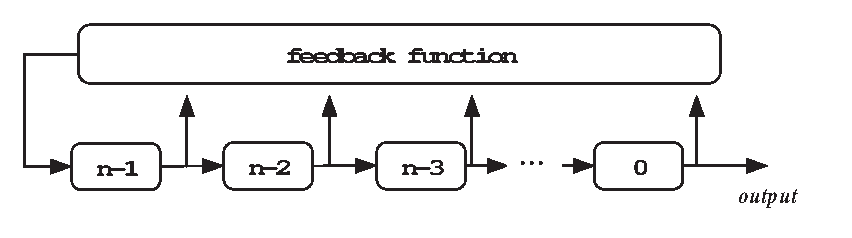
\includegraphics[width=3in]{fsr.eps}
\caption{The Fibonacci NLFSR}
\label{fsr}
\end{figure}
\begin{figure}
\centering
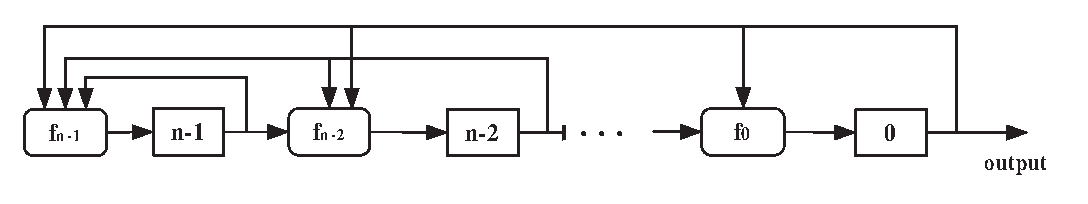
\includegraphics[width=3in]{Galois.eps}
\caption{The Fibonacci NLFSRs}
\label{gsr}
\end{figure}

\section{preliminaries}
In this section, we first review the STP of matrices briefly. Then the multi-linear
form of Boolean function that is obtained by using the semi-tensor product is recalled. Finally, we regard $(n,k)$ NFSRs as a BN. Based on STP, $(n,k)$ NFSRs are converted into a multi-linear form. We first give some notations which will be used in this paper.
\begin{itemize}
  \item $\mathcal{D}=\{0,1\}$.
  \item $I_n:$ the identity matrix of dimension $n$.
  \item $\delta^i_{2^n}:$ the $i$-th column of identity matrix $I_n$.
  \item $\Delta_{2^n}=\{\delta^i_{2^n}|i=1,2,3,...,2^n\}$.
  \item $\mathcal{L}_{n\times m}:$ the set of $n\times m$ matrices, whose column belong to $\Delta_{n}$. For a matrix $L\in\mathcal(L)_{n\times m}$, and $L=[\delta^{i_1}_{n}~ \delta^{i_2}_{n}~ ... ~ \delta^{i_m}_{n}]$, we write $L=\delta_{2^n}[i_1~ i_2~ ... ~ i_m]$ for simplicity. \item $col_i(L):$ the $i$-th column of matrix $L$.
  \item $col(L):$ the set of all column of matrix $L$.
  \item $\mathbb{R}:$ the set of all real number.
  \item $N:$ the set of all positive integers.
  \item $\star:$ the least common multiple.
  \item $\diamond:$ the greatest common divisor.
  \item $\times:$ Cartesian product.
  \item $|S|:$ the number of elements in set $S$.
\end{itemize}


\subsection{Semi-tensor product of matrices}
In this subsection, the definition of STP is given. The multi-linear form of nonlinear Boolean function is obtained by using the method of STP.

\begin{definition}\label{stp}\cite{Cheng2011Analysis}
Let $A\in\mathbb{R}^{n\times m}$, $B\in \mathbb{R}^{p\times q}$. The \textit{semi-tensor product} of $A$ and $B$ is defined as:
\begin{equation}
A\ltimes B=(A\otimes I_{\frac{l}{m})}(B\otimes I_{\frac{l}{p}})
\end{equation}
where $l$ is the least common multiple of $m$ and $p$.
\end{definition}

Obviously, if $m=p$ in Definition \ref{stp}, then the STP of $A$ and $B$ is reduced to their conventional matrix product $AB$.

We identify $\Delta_{2}\sim \mathcal{D}$ i.e $(\delta^1_2\sim 1,\delta^2_2\sim 0)$, and $\delta^1_2(\delta^2_2)$ is called the vector form of logical value $1(0)$.

\begin{lemma}\label{lemma1}\cite{Cheng2011Analysis}
Any Boolean function $f(x_1,x_2,...,x_n)$ with variables $x_1,x_2,...,x_n\in \Delta_2$ can be expressed as a multi-linear form:
\begin{equation}
f(x_1,x_2,...,x_n)=Fx_1\ltimes x_2\ltimes ...\ltimes x_n.
\end{equation}
where $F\in \mathcal{L}_{2\times 2^n}$ is called the \textit{structure matrix} of $f$, and $F$ can be uniquely expressed as
\begin{equation}
F=\left[
    \begin{array}{cccc}
      s_1 & s_2 & ... & s_{2^{n}} \\
      1-s_1 & 1-s_2 & ... & 1-s_{2^n} \\
    \end{array}
  \right]
\end{equation}
with $[s_1,s_2,...,s_{2^n}]$ being the truth table of $f$, arranged in the reverse alphabet order.
\end{lemma}

In the following, we omit the symbol $\ltimes$ for simplicity.


\subsection{$(n,k)$ NFSR}
An $(n,k)$ NFSR consists $n$ binary memories device called bits. The output of an $(n,k)$ NFSR is the value of the $0$-th bit. An $(n,k)$ NFSR is defined as follows. Let $x_i(t),~0\leq i\leq n-1$ be variable representing the value of the $i$-th bit at time $t$. Let $f_i:\mathcal{D}^k\rightarrow \mathcal{D},$ $1\leq k\leq n$, be the next value function of $i$-th bit. The Boolean function $f_i$ depends on the bit $(i+1)mod$ $n$ and up to $k-1$ other bits. Assume the indexes of other $k-1$ bits relating to function $f_i$ are
 $i_1,i_2,...,i_{k-1}$, $i_j\in \{0,1,...,n-1\}$, $j\in{1,2,...,k-1}$, then the value function of $i$-th bit can be expressed as follows:
 \begin{equation}
 x_i(t+1)=f_i(x_{(i+1)mod~n}(t),x_{i_1}(t),...,x_{i_{k-1}}(t)).
 \end{equation}
  So $(n,k)$ NFSR can be described as a BN shown as follows:
 \begin{eqnarray}\label{nfsr}
 \left\{ \begin{aligned}
&x_0(t+1)=f_0(x_1,x_{0_1},x_{0_2},...,x_{0_{k-1}}),\\
&x_1(t+1)=f_1(x_2,x_{1_1},x_{1_2},...,x_{1_{k-1}}),\\
&\vdots\\
&x_{n-1}=f_{n-1}(x_0,x_{n-1_1},x_{n-1_2},...,x_{n-1_{k-1}}),
\end{aligned} \right.
\end{eqnarray}
where $x_i(t)\in \mathcal{D},~0\leq i\leq n-1, ~t=1,2,...$. Let $x(t)=(x_0(t),x_1(t),...,x_{n-1}(t))$ denote the state of $(n,k)$ NFSR and $f=[f_0,f_1,...,f_{n-1}]$ be the vectorial function.
So system (\ref{nfsr}) can be expressed as follows:
\begin{equation}\label{nfsra}
x(t+1)=f(x(t)).
\end{equation}

\begin{definition}
\begin{enumerate}
  \item A state $x_0$ is called an $equilibrium$ $state$ of $(n,k)$ NFSR (\ref{nfsra}), if $fx_0=x_0$.
  \item {$x_0,f(x_0),...,f^p (x_0)$} is called a cycle of $(n,k)$ NFSR (\ref{nfsra}) with length $p$, if $f^p (x_0)=x_0$, and the elements in set \{$x_0,f(x_0),...,f^p (x_0)$\} are distinct.
\end{enumerate}
Let $R(x)$ denote the set of states which can reach state $x$. Let $R^k(x)$ denote the set of states which can reach state $x$ after in $k$ steps.
\end{definition}
Next, we give the definition of $globally$ $stable$, $locally$ $stable$ and the period of $(n,k)$ NFSR.
\begin{definition}
$(n,k)$ NFSR (\ref{nfsra}) is called $globally$ $stable$ with respect to (w.r.t.) the equilibrium state $x_0$, if for any state $x\in \mathcal{D}^n$, there exist a positive integer $N$ such that $f^Nx=x_0$.
\end{definition}

\begin{definition}
$(n,k)$ NFSR (\ref{nfsra}) is called $locally$ $stable$ w.r.t. the equilibrium state $x_0$, if there exist some states $x\in  \mathcal{D}^n\setminus x_0$, such that $f^Nx=x_0$ for some positive integer $N$.
\end{definition}


By using Lemma \ref{lemma1}, we can obtain that $x_i(t+1)=F_i\ltimes^{n-1}_{i=0} x_i(t)$, where $F_i\in \mathcal{L}_{2\times 2^n}$, then the BN (\ref{nfsr}) can be converted into following system:
\begin{equation}\label{nfsr1}
x(t+1)=Lx(t),~t\in N,
\end{equation}
where $x(t)=x_0(t)\ltimes x_1{t}\ltimes ...\ltimes x_{n-1}(t) \in \Delta_{2^n}$ is the state at time $t$, and $L\in \mathcal{L}_{2^n\times2^n}$, $col_i(L)=\ltimes^{n-1}_{i=0}col_i(F_i)$.

\begin{definition}\cite{Dubrova2008On}
The period of an $(n,k)$ NFSR is the length of the longest cyclic output sequence it produces.
\end{definition}

To better study the period of $(n,k)$ NFSR, we propose the definition of minimal period of output sequence of a state in cycle of $(n,k)$ NFSR.
\begin{definition}
For arbitrary state $x$ in a cycle $\mathcal{C}$ with length $l_{\mathcal{C}}$ of an $(n,k)$ NFSR, the minimal period of output sequence $O_x=\{O_1,O_2,...\}$ of $x$ as an initial state is the minimal positive integer $p_x$ such that $O_i=O_{i+kp_x}$, $k=1,2,3,...$.
\end{definition}

\begin{remark}
For simplification, in the following, the output sequence of $x$ means that the output sequence of $x$ as an initial state, and $x$ is in a cycle of $(n,k)$ NFSR.
\end{remark}
In order to investigate the cycle of an $(n,k)$ NFSR, we need the following definition.
\begin{definition}
For an $(n,k)$ NFSR, if the state $x$ is shifted to the state $y$, then the state $x$ is called the $predecessor$ of state $y$, while state $y$ is called the $successor$ of state $x$. The state without predecessor is called a $starting~ state$.
\end{definition}
Let $S$ denote the set of starting states of $(n,k)$ NFSR (\ref{nfsra}).

\section{main results}
In this section, the stability of system (\ref{nfsr1}) is firstly investigated. Then the period of output sequence of system (\ref{nfsr1}) is studied. At last, we investigate the period of output sequence of an composed $(n,k)$ NFSR.

\subsection{Stability of $(n,k)$ NFSR}

Clearly, in an $(n,k)$ NFSR, the equilibrium state can be any state. Assume the equilibrium state of $(n,k)$ NFSR is $\delta^i_{2^n}\sim (i_0,i_1,...,i_{n-1})$. We can make a coordinate transformation
 \begin{eqnarray}\label{nfsr}
 \left\{ \begin{aligned}
&y_j=\neg x_j,~i_j=1,\\
&y_j=x_j,~i_j=0,\\
\end{aligned} \right.
\end{eqnarray}
then system (\ref{nfsr1}) is converted into a system with equilibrium state $\delta^{2^n}_{2^n}\sim(0,0,...,0)$ as follows:
\begin{equation}\label{nfsr2}
y(t+1)=\bar{L}y(t),
\end{equation}
where $y(t)=\ltimes^{n-1}_{i=0}y_i(t)$. Then equilibrium state of system (\ref{nfsr2}) is $\delta^{2^n}_{2^n}\sim(0,0,...,0)$.

Since the form of system (\ref{nfsr1}) is similar to the form of system in \cite{Zhong2014Stability}, we can obtain the same result about the global stability of system (\ref{nfsr1}).

\begin{theorem}\label{th1}
$(n,k)$ NFSR (\ref{nfsr2}) is globally stable with respect to state $\delta^{2^n}_{2^n}$ if and only if there exist a positive integer $1\leq N\leq 2^n-1$ such that $col(L^N)=\delta^{2^n}_{2^n}$.
\end{theorem}

From Theorem \ref{th1}, we can obtain the following corollary.

\begin{corollary}
$(n,k)$ NFSR (\ref{nfsr2}) is globally stable with respect to  $\delta^{2^n}_{2^n}$, if and only if $R(\delta^{2^n}_{2^n})=\Delta_{2^n}$.
\end{corollary}

\begin{remark}
If an $(n,k)$ NFSR is globally stable to $\delta^{2^n}_{2^n}$, then for any state, it can reach state $\delta^{2^n}_{2^n}$ at most $2^n$ steps.
\end{remark}

\begin{theorem}
$(n,k)$ NFSR (\ref{nfsr2}) is locally stable with respect to state $\delta^{2^n}_{2^n}$ if and only if there exist state $x\in \Delta_{2^n} \setminus \delta^{2^n}_{2^n}$ and a positive integer $1\leq N\leq 2^n-1$ such that $L^Nx=\delta^{2^n}_{2^n}$. (i. e there exist state $x\in \Delta_{2^n} \setminus \delta^{2^n}_{2^n}$ which can reach equilibrium state $\delta^{2^n}_{2^n}$.)
\end{theorem}


In the next, we will give an algorithm to decide if an $(n,k)$ NFSR is globally stable under the knowledge of state transition matrix of an $(n,k)$ NFSR.
\begin{algorithm}\label{algorithm1}
\caption{The global stability of an $(n,k)$ NFSR.}
\begin{algorithmic}[1]
\STATE initial set $\Delta=\{1,2,...,2^n\}$
\FOR { $i=1$ to $2^n$}
\FOR { $j=1$ to $2^n$}
\IF  {$col_j(L)=\delta^{2^n}_{2^n}$}
\STATE $R^i(\delta^{2^n}_{2^n})=R^i(\delta^{2^n}_{2^n})\cup \delta^j_{2^n}$
\ENDIF
\ENDFOR
\IF {$R^{i-1}_{\delta^{2^n}_{2^n}}=R^{i}_{\delta^{2^n}_{2^n}}$}
\STATE $num=i-1$
\STATE \textbf{break}.
\ENDIF
\ENDFOR
\IF {$R^{num}_{\delta^{2^n}_{2^n}}=\Delta_{2^n}$}
\STATE the $(n,k)$ NFSR is globally stable.
\ELSE
\STATE the $(n,k)$ NFSR is not globally stable.
\ENDIF
\end{algorithmic}
\end{algorithm}


\begin{lemma}
The set of starting states of an $(n,k)$ NFSR (\ref{nfsr1}), $S$ is equal to $\Delta_{2^n}\setminus col(L)$.
\end{lemma}

In the next, we will give an algorithm to find all cycles of $(n,k)$ NFSR (\ref{nfsr1}).
We firstly give some notations in Algorithm 2. $S_i$ denote the $i$-th state in set $S$.
$V_i$ denotes the set of states which start from state $S_i$ have been visited. $V^k_i$ denotes the $k$-th element in set $V_i$.
$\mathcal{C}_i$ denote the $i$-th cycle of $(n,k)$ NFSR.
 In Algorithm 2, we will firstly find the cycles which start from starting states. Then the cycles without branches will be found.

\begin{algorithm}\label{al1}
\caption{All cycles of $(n,k)$ NFSR (\ref{nfsr1})}
\begin{algorithmic}[1]
\STATE Initialize set $V_i=\varnothing$
\FOR {$i=1$ to $|S|$}
\STATE $V_i=S_i$
\STATE $x=S_i$
\FOR {$j=1$ to $2^n$}
\STATE  $x=Lx$
\IF  {$x\notin V_i$}
\STATE $V_i=V_i\cup x$
\IF {$i>1$ and $x\in V_{i-1}\cup V_{i-2}\cup...\cup V_{1}$}
\STATE \textbf{continue}
\ENDIF
\ELSE
\STATE There exist $V^k_i$ such that $V^k_i$ equal to $x$
\STATE The $i$-th cycle of $(n,k)$ NFSR is $\mathcal{C}_i=\{V^k_i,V^{k+1}_i,...,V^{j-1}_i\}$.
\STATE \textbf{continue}
\ENDIF
\ENDFOR
\ENDFOR
\STATE $Re=\Delta_{2^n} \setminus V_1\cup V_2\cup...\cup V_{|S|}$
\STATE $i=0$
\WHILE {$Re\neq \varnothing$}
\STATE $i=i+1$
\STATE Let $x$ denote the first number of set $Re$, there exist $L^k x=x$.
\STATE The $|S|+i$-th cycle is $\mathcal{C}_{|S|+i}=\{x,Lx,...,L^{k-1}x\}$
\STATE $Re=Re\setminus \mathcal{C}_{|S|+i}$
\ENDWHILE
\end{algorithmic}
\end{algorithm}

\subsection{The period of $(n,k)$ NFSR}
In this section, we firstly give the following lemma before investigating the period of $(n,k)$ NFSR.

Since the number of states in an $(n,k)$ NFSR is finite, we can obtain the following lemma.
\begin{lemma}\label{lemma2}
For arbitrary initial state $\delta^i_{2^n}$ of an $(n,k)$ NFSR, $\delta^i_{2^n}$ always can reach a cycle or an equilibrium point.
\end{lemma}

From Lemma \ref{lemma2}, in the following, we only need to investigate the output sequence of state within a cycle. So in this paper, the minimal period of output sequence of a state in $(n,k)$ NFSR means that the minimal period is only for the states within a cycle of $(n,k)$ NFSR.

In the following, we will provide Algorithm 3 to compute the minimal period of the output sequence of a state in an $(n,k)$ NFSR. Before presenting Algorithm 3, we give a theorem to show the relationship between the period of output sequence of the state in a cycle and the length of the cycle of an $(n,k)$ NFSR.

\begin{theorem}\label{th2}
If the length of a cycle $\mathcal{C}=\{e_0,e_1,...,e_{l-1}\}$ in $(n,k)$ NFSR (\ref{nfsr1}) is $l$, then the minimal period of output sequence of cycle $\mathcal{C}$ is one of the divisor of $l$, and the minimal period of output sequence of every state $e_i,$ $0\leq i\leq l-1$ in cycle $\mathcal{C}$ is equal to the minimal period of output sequence of cycle $\mathcal{C}$.
\end{theorem}
\begin{proof}
Let $p_{\mathcal{C}}$ denote the minimal period of the output sequence of cycle $\mathcal{C}$, and let $p_i$ denote the minimal period of output sequence of initial state $e_i$, and $l_i$ denote the output sequence of initial state $e_i$. Let $O_{\mathcal{C}}=\{O^0_{\mathcal{C}},^1_{\mathcal{C}},...,O^{l-1}_{\mathcal{C}}\}$ with length $l$ denote the output sequence of cycle $\mathcal{C}$ which start at state $e_0$.

Because $\mathcal{C}$ is a cycle, $l$ is one of period of the output sequence of cycle $\mathcal{C}$. Apparently, the multiple of $l$ is the period of output sequence of cycle $\mathcal{C}$. We also can know that one of the divisor of $l$ can be the period of the output sequence of cycle $\mathcal{C}$.
Since $e_i\in \mathcal{C}$, $p_i$ must be a divisors of $l$. The output sequence of $e_i$ is equivalent to the output sequence of cycle $\mathcal{C}$ after $i$ times shifts. So the minimal period of output sequence $e_i$ is equal to $p_{\mathcal{C}}$.
\end{proof}

From Theorem $\ref{th2}$, we can know that the minimal period of every state in a cycle is the same, so the investigation of minimal period of output sequence of a state can be called the investigation of minimal period of a cycle of an $(n,k)$ NFSR.

Now, based on Theorem \ref{th2}, we give an algorithm to compute the minimal period of output sequence of an initial state of $(n,k)$ NFSR (\ref{nfsr1}). The following algorithm is based on the fact that all cycles of $(n,k)$ NFSR (\ref{nfsr1}) are known. Algorithm 3 can be used to find out the period  of output sequence of given cycle. For the given cycle, the length of the cycle is denoted by $l$, and the period of the output sequence of the cycle is denoted by $p$. Algorithm 3 only can compute the minimal period of output sequence of a cycle. So if we want to compute the minimal period of all cycles, Algorithm 3 should be used repeatedly.
%and all the cycle of $(n,k)$ NFSR are denoted by $\mathcal{C}_1,\mathcal{C}_2,...\mathcal{C}_s$ with length $l_1,l_2,...,l_s$, where $s$ denote the number of $(n,k)$ NFSR. Let $d^i_j$ denote the $i$-th divisor of $l_j$.


%In the following, we provide an algorithm to compute the minimal period of output sequence of a cycle of $(n,k)$ NFSR. We firstly introduce some notation which will be used in the following algorithm.

\begin{algorithm}\label{algorithm2}
\caption{The period of output sequence of a cycle of $(n,k)$ NFSR (\ref{nfsr1}).}
\begin{algorithmic}[2]
\STATE initial $p=l$
\FOR { $i=1$ to $l$}
\STATE flag=true
\IF {$i$ is a divisor of $l$}
\STATE $I_1$ is a subsequence which formed by the $1$-th element to $i$-th element of cycle $\mathcal{C}$
\FOR {$j=1$ to $l/p-1$}
\STATE $I_2$ is a subsequence which formed by the $j\ast i$-th element to $(j+1)\ast i-1$-th element of cycle $\mathcal{C}$.
\IF {$I_1\neq I_2$}
\STATE flag=false
\ENDIF
\ENDFOR
\ENDIF
\IF {flag=true}
\IF {$i<p$}
\STATE $p=i$
\ENDIF
\ENDIF
\ENDFOR
\end{algorithmic}
\end{algorithm}

So the period of $(n,k)$ NFSR (\ref{nfsr1}) can be found by the following steps:
\begin{itemize}\label{period}
  \item Finding all cycles of the $(n,k)$ NFSR (\ref{nfsr1}).
  \item Finding the minimal periods of all cycles of the $(n,k)$ NFSR (\ref{nfsr1}) by using Algorithm 3.
  \item Finding the maximum value of minimal periods of all the cycles of $(n,k)$ NFSR (\ref{nfsr1}).
\end{itemize}

\section{examples}
In this section, we give two examples to illustrate our theoretical results.
\begin{example}
Consider an $(3,3)$ NFSR with following equations:
\begin{eqnarray}\label{ex1}
 \left\{ \begin{array}{lcl}
x_0(t+1)&=&(x_0(t)\wedge x_2(t))\vee (\neg x_0(t)\wedge x_1(t)),\\
x_1(t+1)&=&(x_0(t)\wedge (\neg x_1(t)\vee \neg x_2(t)))\vee(\neg x_0(t)\\
&&\wedge(\neg x_1(t)\wedge x_2(t))),\\
x_{2}(t+1)&=&(x_0(t)\wedge (\neg x_2(t)\wedge \neg x_1(t)))\vee(\neg x_0(t)\\
&&\wedge(\neg x_1(t)\vee \neg x_2(t)))
\end{array} \right.
\end{eqnarray}
By using the method of STP, we can transfer system (\ref{ex1}) into following multi-linear form:
\begin{equation}
x(t+1)=L_1x(t),
\end{equation}
where $L_1=\delta_{8}[4~6~2~5~8~7~1~3]$, $x(t)=x_0(t)x_1(t)x_2(t)\in \Delta_{2^3}$.

In $(n,k)$ NFSR (\ref{ex1}), there is no equilibrium state, so it is not globally stable or locally stable.

We know that there is a cycle of $(n,k)$ NFSR (\ref{ex1}), and the cycle is $\delta^1_8\rightarrow \delta^4_8\rightarrow \delta^5_8\rightarrow \delta^8_8\rightarrow \delta^3_8\rightarrow \delta^2_8\rightarrow \delta^6_8\rightarrow \delta^7_8\rightarrow \delta^1_8$. The output sequence of the cycle is $11001100...$. The period of this output sequence is $4$, which is coincident with the result of Theorem {\ref{th2}}. So we can conclude that the period of $(n,k)$ NFSR (\ref{ex1}) is 3.
\end{example}

\begin{example}
Consider an $(3,3)$ NFSR with following equations:
\begin{eqnarray}\label{ex2}
 \left\{ \begin{array}{lcl}
x_0(t+1)&=&(x_0(t)\wedge \neg x_2(t))\vee (\neg x_0(t)\wedge x_1(t)\wedge 1),\\
x_1(t+1)&=&(x_0(t)\wedge (\neg x_1(t)\vee x_2(t)))\vee(\neg x_0(t)\wedge \\
&&( x_1(t)\wedge x_2(t))),\\
x_{2}(t+1)&=&(x_0(t)\wedge (x_1(t)\vee \neg x_2(t)))\vee(\neg x_0(t)\wedge\\
&&(\neg x_1(t)\wedge \neg x_2(t))).
\end{array} \right.
\end{eqnarray}
By using the method of STP, we can turn system (\ref{ex1}) into following multi-linear form:
\begin{equation}
x(t+1)=L_2x(t),
\end{equation}
where $L_2=\delta_8[5~3~6~1~2~4~8~7]$, $x(t)=x_0(t)x_1(t)x_2(t)\in \Delta_{2^3}$.
In $(n,k)$ NFSR (\ref{ex2}), there is no equilibrium state, so $(n,k)$ NFSR (\ref{ex2}) is not globally stable or locally stable.

We can know that there are two cycles denoted by $\mathcal{C}_{21}, \mathcal{C}_{22}$. $\mathcal{C}_{21}=\delta^1_8\rightarrow \delta^5_8\rightarrow \delta^2_8\rightarrow \delta^3_8\rightarrow \delta^6_8\rightarrow \delta^4_8\rightarrow \delta^1_8$, $\mathcal{C}_{22}=\delta^7_8\rightarrow \delta^8_8\rightarrow\delta^7_8$. The output sequence of $\mathcal{C}_{21}$ is $101101101101...$. The output sequence of $\mathcal{C}_{22}$ is $00...$. So we can know that the minimal period of output sequence of $\mathcal{C}_{21}$ is $3$, and the minimal period of output sequence of $\mathcal{C}_{22}$ is 1.
So we can get that the period of $(n,k)$ NFSR (\ref{ex2}) is 3.
\end{example}



\section{conclusion}
This paper investigated the stability of $(n,k)$ NFSR, the period of $(n,k)$ NFSR and the period of composed $(n,k)$ NFSR. First, we treated the $(n,k)$ NFSR as a BN. By using the method of STP, the $(n,k)$ NFSR was transformed into a multi-linear system. Then an algorithm was proposed to judge the stability of an $(n,k)$ NFSR. After that, we proposed an algorithm to find the minimal period of output sequence of a cycle of an $(n,k)$ NFSR. Finally, two examples were given to verify the results obtained in this paper.

\section*{Acknowledgment}
This work was supported by the National Natural Science Foundation of China under Grant No. 61573102, and China Postdoctoral Science Foundation under Grant No. 2014M560377 and 2015T80483, Jiangsu Province Six Talent Peaks Project under Grant 2015-ZNDW-002.

\bibliographystyle{ieeetr}
\bibliography{F:/conference_paper_reduced/referencee}
\end{document}
